\clearpage
\twocolumn[{\centering\large\bfseries Supplemental Material\par\vspace{0.5em}}]
\renewcommand{\theHsection}{supp.\arabic{section}}
\renewcommand{\theHsubsection}{supp.\arabic{section}.\arabic{subsection}}
\renewcommand{\theHtable}{supp.\arabic{table}}
\renewcommand{\theHfigure}{supp.\arabic{figure}}
\setcounter{section}{0}
\setcounter{subsection}{0}
\setcounter{table}{0}
\setcounter{figure}{0}
\renewcommand{\thetable}{S\arabic{table}}
\renewcommand{\thefigure}{S\arabic{figure}}


\noindent\textit{References: main-paper numbering.}\par
\section{Parameter efficiency}
\begin{table}[t]\centering
\caption{The total number of parameters within models and proportion trainable is given in Supplemental Table S1. Training only classifier head not included.}
\label{tab:checked2}
\footnotesize\setlength{\tabcolsep}{2pt}
\sbox{\uploadedtablebox}{\begin{tabular}{llll}\toprule
ID & Total Parameters & Trainable Parameters & (\%) Trainable\\\midrule
M0 & 87171072 & 590592 & 0.68\\
M1 & 87613440 & 1032960 & 1.18\\
M2 & 175226880 & 2065920 & 1.18\\
M3 & 175226880 & 2065920 & 1.18\\
M4 & 175424257 & 2263297 & 1.29\\
\bottomrule\end{tabular}}
\ifdim\wd\uploadedtablebox>\columnwidth\resizebox{\columnwidth}{!}{\usebox{\uploadedtablebox}}\else\usebox{\uploadedtablebox}\fi
\end{table}
M0 has 590k trainable parameters. M2 contains unused full face modality. 1,032,960 parameters are trainable. 2,065,920 is the nominal trainable parameter count of the instantiated model. The 128 class training only head has 98,432 parameters and is not included in this table. Across all adapted models, the maximum number of trainable parameters is 2.26M (1.29\%), within a double encoder model (175M). Hardware details, available runtimes, software versions, and checkpoint hashes are recorded in artifact. Maximum memory consumption was not taken.\par

\begin{table}[t]\centering
\caption{Average weighting in face branch for each protocol and seed. Standard deviation (in brackets) within endpoints. Weights are descriptives and do not indicate reliable calibrated detection.}
\label{tab:checked10}
\footnotesize\setlength{\tabcolsep}{2pt}
\sbox{\uploadedtablebox}{\begin{tabular}{llll}\toprule
Protocol & Seed 7 & Seed 42 & Seed 123\\\midrule
Masked & 0.712 (0.118) & 0.709 (0.100) & 0.749 (0.092)\\
Sunglasses & 0.841 (0.082) & 0.825 (0.083) & 0.830 (0.082)\\
Neutral & 0.773 (0.107) & 0.767 (0.096) & 0.778 (0.099)\\
MFR2 & 0.659 (0.118) & 0.632 (0.117) & 0.696 (0.103)\\
RMFRD & 0.745 (0.086) & 0.697 (0.090) & 0.775 (0.071)\\
\bottomrule\end{tabular}}
\ifdim\wd\uploadedtablebox>\columnwidth\resizebox{\columnwidth}{!}{\usebox{\uploadedtablebox}}\else\usebox{\uploadedtablebox}\fi
\end{table}
\section{Execution and recovery records}
Execution environment: PyTorch (version 2.14.0+cpu), deterministic. DINOv2 was cached. Checkpoints are atomic containing optimiser state, ordered data samples, next batch index, loss in current epoch, and random number generator states in Python, NumPy and PyTorch. Incompatible checkpoints cannot be resumed, due to manifest and source signature. In order to save a run in the serial co-ordinator, all scored hash checks must be complete. Periocular only training means that full face modality was never used in training. This means that random numbers were used differently to historical trainer. Therefore it cannot be claimed that identical bitwise optimisation was performed.\par
\section{Reproducibility details}
To reproduce this work licensed data must be obtained. The correct facial/periocular paths must be recreated. Frozen training and pair manifests must be verified. The software as recorded, and DINOv2 cache must be set up. The CPU coordinator must be run. All models will be trained for 5 epochs. Models will be scored for each protocol. Model summaries will only be created once all evaluations have been performed. File locking has been implemented to prevent multiple instances of the coordinator running. Multiple runs will produce verified complete runs. If the experiment is interrupted, it will resume from a checkpoint of the atomic optimiser and random number generator. Face images, pre-trained weight binaries and approximately 8.6 GB of newly trained checkpoints are not included. Checksums of these files are provided for local lineage checking. To reproduce inference, access to binaries must be provided.\par
Mathematical checks can be made without torch, images and checkpoints. The verification script in this repository recreates ROC scores, checks alignment and checksums of pairs, recalculates mean/SD of seeds, and checks values in the table of the manuscript. 90 historic metric files, sensitivities and corrected historic MFR2 inferences have been saved. If all of these pass, all files are internally consistent. However, no guarantees can be made that this work is novel, accepted for publication, and that images have semantically correct labels.\par
Historic versions of this manuscript and follow-up work can be found in the history folder. Claims or numerically tabulated data within these files are now out-of-date with the full CPU experiment in this paper. No new training is represented by filtered scores in historic files. Incomplete training or smoke runs do not produce headline tables. Large blocks of text and vector figures in both IEEE and arXiv are re-created together using complete evidence from results.\par
\section{Additional interpretation and result records}
In all test protocols, whole face LoRA performs better than frozen projection models, supporting hypothesis H1. The greatest improvements were seen in MFR2 and masked ROF. However, smaller improvements were found in RMFRD. Supervised adaptation thus appears to be beneficial in this experiment. It cannot be determined that adapting general visual encoders (as opposed to face specific pre-trained models) is beneficial in this experiment.\par
Depending on the area of the face shown, RQ2 is somewhat supported. Periocular LoRA has the best results in masked, but performs poorly in sunglasses and loses useful information in neutral. Therefore H2 is only somewhat supported. Upper face features provide useful information for distinguishing between subjects in lower face occlusion scenarios. However, they do not provide a good representation in all 3 conditions. Using fixed fusion provides a good baseline since information in both regions can be preserved without learning a weighting policy.\par
From results in SFace, it appears that greater ranking performance can be achieved by training the model specifically on faces. However, due to differences in training data and alignment, a fair comparison of model architectures could not be made. Therefore this work should be considered as an ablation study and study of reproducibility. In order to claim competition within face recognition, comparisons must be made with equivalent baseline models, with more identities and verified labels.\par
Since a constant auxiliary vector is used, care must be taken in the interpretation of results. As input descriptors are provided, no measure of variable quality is present in this experiment. Although the gate can react to embeddings, no evidence can be provided that quality cues improve performance. Future work using quality cues should be designed with validated descriptors and controlled ablation studies on descriptors. Evaluation criteria should also be fixed before investigation.\par
Records for 15 models in the grid have been included. 120 ordered raw-score files across 8 validation/test/external protocols. Evaluation reports, final training progression information, checksums of checkpoints and a table summarising 5 conditions with 25 rows. 10 comparisons of AUC in pairs with 3 seeds. Variance in AUC between seeds, bootstrap and conditional confidence intervals is included. Fixed versions of trainer, evaluator, common utilities, models and metrics have been included. Checksums are provided for each. If any of these sources change, execution signatures will become invalid.\par
\section{Same-branch comparison context}
As different weights are applied in the fixed and gated fusion models, different features are being learnt in each branch. By applying different weights to the gated models, but keeping the same branches, it was found that equal weighting in the gated branches performs better than learned weighting in masked ROF pairs. This analysis allows understanding of whether representations are useful, or inferences are useful. However, no assumptions are made on whether representations and inferences will be useful in tandem.\par
\section{Extended interpretation and source-image review}
The methods used to produce fusion, LoRA and weighted models are well known. Given the methods proposed in FRoundation and recent implementations using DINOv2-LoRA periocular [25, 30], it can no longer be claimed that the novel contribution of this work is adaptation within the backbone model. However, it is still valuable to understand whether the same level of robustness can be achieved using regional features, weights and thresholds. If two joint models perform competitively, it cannot be concluded that the weight adaptation is responsible for the performance difference. Having same branch control models provides a better indication of this.\par
Score distribution plots show the overlapping of genuine and impostor scores. However, no information on which identities or why errors were made can be seen. Manual inspection of labelled identities in licensed source data must be performed to make qualitative decisions. From retaining manifests and exclusion ledgers, this can be done without distributing private or restricted face images in the repository.\par
Since a constant auxiliary vector is used, care must be taken in the interpretation of results. As input descriptors are provided, no measure of variable quality is present in this experiment. Although the gate can react to embeddings, no evidence can be provided that quality cues improve performance.\par

\section{Inference architecture}
\begin{figure}[t]\centering
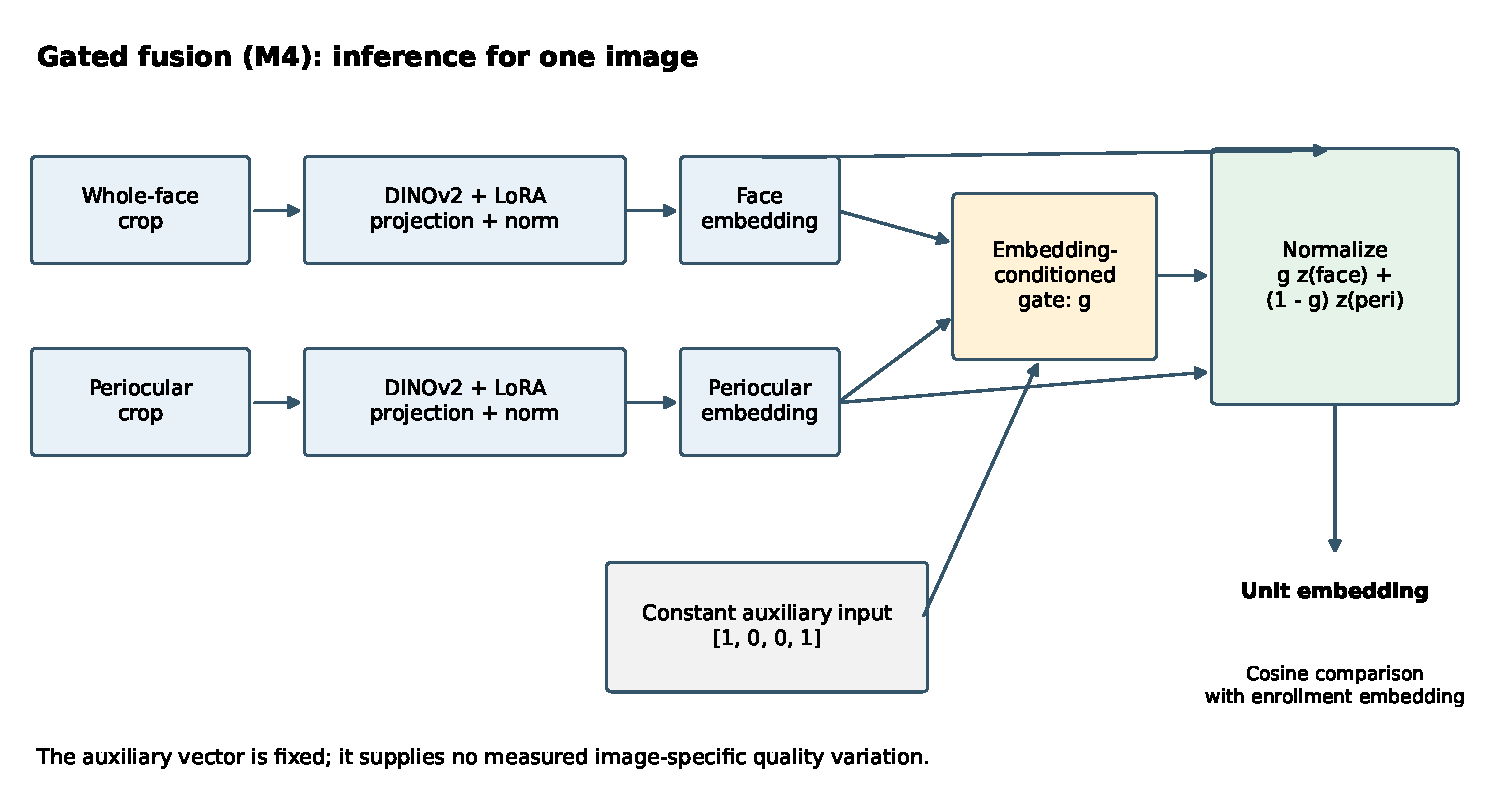
\includegraphics[width=\columnwidth]{fig_gated_architecture.pdf}
\caption{Gated-fusion inference path for one image. Both branch embeddings and the constant auxiliary vector feed the gate; the weighted mixture is normalised. The enrolment image follows the same model before cosine comparison. The training-only identity classifier is omitted from the inference path.}\label{fig:supparchitecture}\end{figure}


\section{SFace preprocessing controls}
Shared-crop SFace preprocessing control. The exact DINOv2 whole-face input files were resized to 112-by-112 pixels for SFace, without YuNet detection or landmark alignment. AUCs were 0.8408, 0.7775, 0.8689, 0.9513, and 0.6532 in the same protocol order (Supplemental Table S3); all 3402 unique images were extracted without failure. The two SFace protocols use different preprocessing, so their AUCs are preprocessing diagnostics rather than directly interchangeable baseline results. Neither is a matched-training comparison with DINOv2 because architecture, pretraining, resolution, and supervision differ.\par
\begin{table}[!ht]\centering\footnotesize\setlength{\tabcolsep}{2pt}
\caption{Separate SFace preprocessing protocols on the same retained pair lists. AUCs include failed pairs at score -1. Failed-pair counts are shown separately for each protocol. Table IX of the main paper reports only the aligned diagnostic.}
\label{tab:sfaceshared}\begin{tabular}{lrrrr}\toprule
Protocol & Aligned AUC & Failed & Shared AUC & Failed\\\midrule
Masked ROF & 0.9399 & 9 & 0.8408 & 0\\
Sunglasses ROF & 0.9440 & 48 & 0.7775 & 0\\
Neutral ROF & 0.9991 & 0 & 0.8689 & 0\\
MFR2 & 0.9968 & 0 & 0.9513 & 0\\
RMFRD & 0.8187 & 1155 & 0.6532 & 0\\
\bottomrule\end{tabular}\end{table}

\section{Data provenance and ethics records}
This study uses existing ROF, MFR2, and RMFRD datasets. Project workflows and captured run paths identify Kaggle-hosted execution copies; the original sources are the ROF repository, the MFR2 maintainer page, and the RMFRD repository. The local ROF annotation snapshot matches the audited upstream files, but a complete image-acquisition log was unavailable. Source identifiers and exclusion ledgers are retained.\par
The ROF repository carries an MIT license for software and associated documentation. The MFR2 maintainer page mentions a Creative Commons license without identifying its specific version or terms in the inspected text. The inspected RMFRD README describes web collection and supplies downloads, but an explicit image-use license was not located there. These records do not establish permission for every underlying photograph or a definitive redistribution rule for every image. The release therefore excludes source face-image binaries and trained checkpoint binaries; it provides code, manifests, hashes, derived scores, and manuscript figures.\par
No project-specific institutional approval, formal exemption, or participant-consent documentation was located in the records reviewed. This is a documentation limit; it does not establish that review was unnecessary or that consent was absent. No approval number, exemption, consent claim, or blanket image permission is inferred from public availability. The factual ethics-review determination and outstanding dataset/image-use permissions remain unresolved.\par
Source records checked on 22 November 2026: \href{https://github.com/ekremerakin/RealWorldOccludedFaces}{ROF repository}, \href{https://github.com/ekremerakin/RealWorldOccludedFaces/blob/main/LICENSE}{ROF license}, \href{https://sites.google.com/view/masktheface/mfr2-dataset}{MFR2 maintainer page}, \href{https://github.com/X-zhangyang/Real-World-Masked-Face-Dataset}{RMFRD repository}.\par
